\documentclass[11pt]{book}
\usepackage{graphicx}
\usepackage[margin=1in,bindingoffset=.2in]{geometry}
\usepackage[backend=biber, style=ieee]{biblatex}
\addbibresource{references.bib}
\usepackage[parfill]{parskip}

\begin{document}
\begin{titlepage}
	\newgeometry{margin=1in}
	\begin{center}
		{\huge Advanced Querying and Analysis\\ of Git Repositories\\}
		\vspace{1.5cm}
		{\Large \textbf{Daniel Brown} \\}
		{\Large Department of Computer Science, University of York \\}
		\vspace{1.5cm}
		
\includegraphics[width=100px]{images/university-of-york-shield} \\
		\vspace{1.5cm}
		{\Large September 2015 \\}
		\vspace{1.5cm}
		\Large Supervised by Dr. Dimitris Kolovos \\
		\vspace{1.5cm}
		\Large A thesis submitted in partial fulfilment for the degree of \\ \textit{Master of Science in Advanced Computer Science}\\
		\vspace{5cm}
		\small XX,XXX words as counted by the `detex thesis.tex | wc -d` unix commands
	\end{center}
	\restoregeometry
\end{titlepage}

\chapter*{\centering Abstract}
\addcontentsline{toc}{chapter}{Abstract}
\begin{center}
	\parbox{350pt}{
Git is one of the most popular version control systems available \cite{gitpopularity} and, as well as many privately hosted instances, powers the well-known social programming website GitHub \cite{gitpowersgithub}.

Despite Gits popularity there are few systems available for analysing a git repository or querying it for useful metrics such as most popular commit time, largest commit, most active contributor or something more complex.

The systems that do exist to analyse Git repositories, namely GitInspector \cite{gitinspector} and Github, don't allow for custom queries to be written by the user. Meaning, for example, you cannot ask the question "What day of the week is Daniel most likely to author a commit of over 100 lines" or "Which contributor has had the highest percentage of their committed lines changed by someone else". 

This project presents a tool, called EpsilonGit, which allow users to write these custom queries by letting them interact with a git object database as a model using the Epsilon platform and its associated domain specific modelling languages. This model-based solution is then compared with existing technologies on the parameters of code complexity, speed, and extensibility by the user.
}
\end{center}

\tableofcontents

\chapter{Introduction and Background}
\label{introandbackground}
\section{Acknowledgement}
I would like to take this opportunity to thank Dr. Dimitris Kolovos who not only provided support and encouragement throughout the course of this project, but also came up with the original idea of using model driven engineering to interact with git and added features into the Epsilon suite to support some of the work I was doing.

A special thank-you is extended to my parents, siblings and girlfriend who have supported me throughout the trials and tribulations of my time at York by visiting both myself and the National Railway Museum an inordinate amount of times. The same gratitude is required of my friends both from at home in Dunstable and The University of Hull, where I completed my Bachelors degree. %The museum bit is an inside joke. I'll keep it in for a laugh

\section{Statement of Ethics}
Ethics in research is of paramount importance and therefore this project has been carried out with them in mind at every step. 

All literature, ideas and code that has been used in the formation of this project has been correctly referenced and credit has been given where it is due.

The data that my project interacts with is a local copy of a git database. The user must source this data on their own, and therefore the project doesn't have to deal with any authentication or security. EpsilonGit only gives people a different view on data they already have.

No other significant ethical issues related to this project could be identified.

\clearpage

\section{Introduction and Background}
% Rough outline of git 
	% (e.g. its a distributed VCS... so people have code locally to be modelled, people use it for x functions (e.g. commit, branch, put their name to code) )
	% Why would someone what to query and analyse their git repository?
	% Some cool questions that could be asked
	
Git is a free and open source distributed version control system \cite{gitintro} that is designed to allow users to manage changes to files, often source files in a software project. This enables developers to "roll back" to a previous version of a file, see the difference between a file at two different times or determine which team member authored a line of code. 

Version control best practices suggest that a developer should be committing code a little at a time and quite often \cite{gitbestpractices}, this makes it a good place to analyse to determine an individual developer or teams working practices in retrospect.

A project manager may want to analyse a git repository to answer questions such as "How large is the average commit size?", "What time of the day are most commits made?" and "Which of my developers is committing the most code that is later replaced?". The answers to these questions may allow improvements in both quality of code and workplace practices.

% Rough outline of modelling
	% What is modelling?
	% Why is it _possibly_ suitable for this project?
Model Driven Engineering is an approach to tackle the complexity of data, and how it is interacted with, through the use of high level abstractions called models \cite{modeldrivenengineering} and a set of Domain-specific modelling languages and Transformation engines and generators.   
	
Due to the large array of features provided by git and the widespread use of hashes and graph data structures in the underlying system it is often considered to be complex \cite{gitcomplex}\cite{githard}\cite{gitmixedmetaphors}.

In this paper it is proposed that a model driven engineering solution to querying and analysing git repositories is a good solution as it removes much of the complexity associated with git.

% Discussion of epsilon
% Discussion of the epsilon driver framework and what integrating with epsilon gets us (e.g. ability to make HTML from models, use of EOL Language, ability to run in and out of eclipse, etc)

Epsilon is a family of languages and tools for code generation, model-to-model transformation, model validation, comparison, migration and refactoring \cite{epsilonhomepage}. Whilst Epsilon comes with support for interacting with EMF, XML and several other types of model formats out-of-the-box it also has a system called the Epsilon Model Connectivity layer which allows developers to implement drivers for other types of models, in this case git.

\section{Motivation}
% Motivation
	% Improve companies, open source projects and individuals understanding of their code and workflows
	% Encourage people to use and invest in Modelling, particularly using epsilon
	% Release it to the world and see what innovative and cool information people could get from their git repositories. With open data and software all kinds of weird shit can be done the original creator wouldn't have thought of.
The Joel Test \cite{joeltest} is often cited as a simple list of best practices for software development. Rule number 1 is to use version control software in order to aid teamwork, maintain a canonical history of source code and reduce the likelihood of losing any work. The positive impact that version control has means that many open source, individual and commercial projects use version control -- one of the most popular being git \cite{gitpopularity}. 

Although many projects use git there are very few tools for querying and analysing the metadata and other information contained within git repositories. Those that are available lack the ability to add user-designed custom queries. 

Through developing a system in which users can write their own custom queries in an easy-to-use and abstract fashion it is thought that teams may be able to learn more about their own workflows and where improvements can be made -- this could be particularly useful to teams using agile methodologies which lack the rigid structure of older methods such as Waterfall.

The software produced as part of this project should also make it easier to determine if git best practices \cite{gitbestpractices} are being followed. In addition to best practices some teams set project wide best practices for commit messages \cite{erlanggitcommitmessages}, users should be able to write validators to ensure these are being used.

As well as helping teams understand their git repositories this project also aims to encourage Software Engineers to learn about and invest in Model-Driven Engineering. It is the the hope of the author that combining MDE with a technology as prevalent as git may help to widen its appeal. In particular it would be great if this attracted more people to the open source Epsilon MDE platform \cite{epsilonhomepage}.

One of the more interesting aspects of the project will be opening up a world of newly accessible data to people and seeing what interesting analysis they can come up with that the author alone wouldn't have thought of.

\section{Aims and objectives}
\label{aimsandobjectives} 
%Aims and objectives
	% Develop a solution which covers all of the most common parts of git (e.g. Object Model, Branches, Authors and Committers)
	% Develop a solution which has as fast or faster runtime for the same output as GitInspector / Github / GitSQL
	% Develop a solution which requires less code, and code of lower complexity for the same output as other solutions
	% Develop a solution which, at the same times, provides high level simple nice clean interaction whilst allowing access to low level stuff for those who also want that interaction
This project aims to implement an Epsilon Model Connectivity (EMC) driver to enable querying and analysis of git repositories from the domain-specific programming languages of the Epsilon Eclipse framework.

The objectives of the project are as follows:

\begin{enumerate}
	\item (Functional) Develop a EMC solution for interacting with the most commons parts of Git (Object Model, Branches and Author \& Committer Information) through Epsilon Eclipse
	\item (Non-Functional) Optimise the solution so that it produces the same output as GitInspector in the same amount of time or less 
	\item (Non-Functional) The solution should allow developers to write queries with identical output to GitInspector and GitHub with less code, and code of less compexity
	\item (Non-functional) The solution should provide access to all low-level properties of the covered areas of git whilst providing higher-level methods to speed up development of user-written queries
\end{enumerate}

\section{Report Structure}
% Report Structure
	% A paragraph or two explaining the overall flow of this document, and calling out the names of each chapter. Not repeating the table of contents, but instead highlighting important sections in prose.

This paper covers the entire process of development of EpsilonGit.

Chapter 2 covers a literature review undertaken before work was carried out, model driven engineering and the git object model are discussed in detail. Using the information ascertained in the literature review chapter 3 discusses the requirements of this project. Chapter 4 discusses several software engineering methodologies that could be followed during the course of development and a decision is made.

Chapter 5 explains the processes undertaken during the design stage, including the interaction between JGit and the Epsilon Model Connectivity layer. The actual implementation details of EpsilonGit are discussed at length in Chapter 6. Chapter 7 rounds up the practical portion of the report by explaining how several types of testing were used together to form a complete testing framework for the EMC driver.

Chapter 8 evaluates the work undertaken against the aims and objectives which were set out in section \ref{aimsandobjectives}. Conclusions from the work are drawn in Chapter 9 and potential future work ideas are provided to the reader. Finally, Chapter 10 reflects on the project as a whole and the author himself.  

\chapter{Literature Review}
% Intro paragraph "This chapter looks at the existing literature... etc"
% Section on literature about Git and the git object model
	% Conclusions drawn from the literature
		% A well known model, with some interesting idiosyncacies. Fits modelling well.
		
\label{litreview}
This chapter looks at the existing literature in the relation to the Git Object Model, Model Driven Engineering techniques, Previous attempts at analysing git repositories and techniques for interacting with object models -- such as the HTML Document Object Model -- which are similar to Git.

\section{Git and Version Control Systems}
\label{sec:git}
Version control systems (VCS) allow Software Engineers to keep a history of changes made to the files they work with. Diomidis Spinellis of Athens University of Economics and Business states that adopting a VCS can be the most important tooling improvement a Software Engineering team can make \cite{toolsofthetrade}.

Git is a version control system originally developed by Linus Torvalds, known for developing the Linux Kernel, with the goals of being fast and efficient with large projects \cite{progit}.

There are two main types of VCS, Centralised Version Control Software and Distributed Version Control Software. Centralised version control systems rely on a central server which contains the canonical source repository whilst distributed systems downloads a complete clone of the repository with a full commit history, meaning each client has a first class repository\cite{whydistributed}.

Distributed version control software has several advantages over centralised systems. Firstly they allow any developer to have write access to a repository, rather than having to submit a patch to someone with committer privileges, which lowers the barrier to entry on open source projects \cite{distributedimpactoss}. Secondly they allow cheap local branching and merging as well as reduced redundant file storage thanks to the use of changesets rather than individual file revisions \cite{distributedimpactoss}. 

Whilst distributed version control systems \cite{whydistributed}, and in particular git \cite{gitpopularity}, have become more popular than centralised version systems there are still some proponents of CVS thanks to the fact that you don't have to download potentially very large repositories with very large histories \cite{cvsvsvcs}.

Git uses the distributed model, meaning each computer on which a repository is used has a complete copy of its history. This makes it a good candidate for analysis as any team member will be able to be involved in the process rather than just the central repository administrator.

Although there are many methodologies for using version control systems all of them contain the same basic commands which form the majority of a users interaction with their VCS. In Git these commands are \cite{gitrefbasic}: 

\begin{table}[h]
\centering
\begin{tabular}{| l | p{9cm} |}
\hline
\textbf{Command} & \textbf{Action} \\ \hline
git clone [remote repository location] & Downloads a repository and all its history from a specified remote location \\ \hline
git add [file] & Adds a file to the git index so that its changes will be tracked \\ \hline
git commit [message] & Stores current changes to history with a message to inform other engineers why changes were made \\ \hline
git push & Sends local changes to a remote repository \\ \hline
\end{tabular}
\caption{Basic Git Commmands}
\label{tab:basic-git-commands}
\end{table}

The git community has developed several different workflows to interact with git for different types of projects and requirements of those projects \cite{gitcomparingworkflows}. 4 such examples are: 

\begin{enumerate}
	\item Centralized Workflow; which works in much the same way as a CVS would
	\item Feature Branch workflow which requires engineers to create a new branch for each feature they are working on before merging back into a main branch which is considered the production ready code
	\item The Gitflow Workflow; which is a mixture of the two previous workflows
	\item Forking Workflow; Commonly used by open source projects. A contributor makes changes in his own local repository and then requests that they be 'pulled' into the main public repository
\end{enumerate}

The many different ways of using git suggest that different analytics may also be required.

\clearpage

\section{The Git Object Model}
The core of git is a content-addressable filesystem which can store any object and assign it a hashcode by which it can be identified \cite{progit}. There are 4 main types of object stored in this system, known as the git object model, which are shown in Figure \ref{fig:gitobjectmodeldiagram}.

\begin{figure}[h]
	\centering
	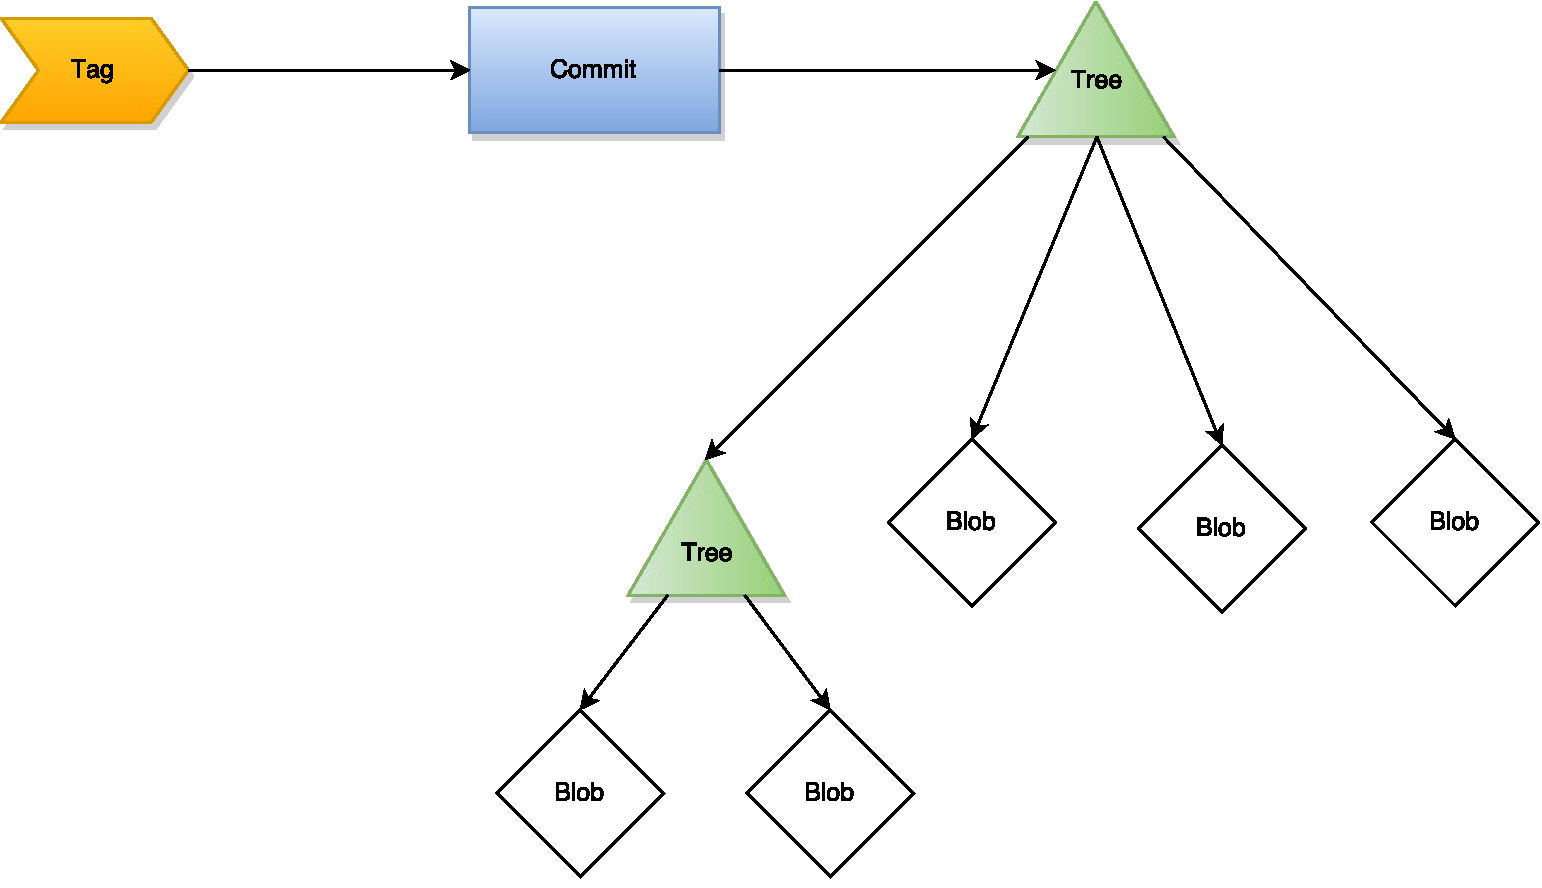
\includegraphics[width=0.7\textwidth]{images/gitobjectmodel}
	\caption{The relationships between Git Objects}
	\label{fig:gitobjectmodeldiagram}
\end{figure} 

Each of these objects will now be discussed in more detail.

\subsection{Blob}
In git a blob is an array of bytes, which can be text or binary data, that is stored in the content-addressable file system. Blobs should not be confused with files as they are just content with no metadata such as filename, in fact if two files are added to git with exactly the same content, and therefore hashcode, they share a blob.

\subsection{Tree}
A tree object in git can be thought of as analogous to a directory in a UNIX file system. For each file in the tree a tuple is stored of the name of file, the hashcode of the blob which contains its content, and a numeric file type code \cite{gitmagic}.

A tree can also contain the names and hashcodes of other trees, allowing for a hierarchical file system, as shown in Figure \ref{fig:gitobjectmodeldiagram}. 

\subsection{Commit}
The commit object type stores information about a snapshot of the blobs and trees in the git repository at a particular time. The information includes the name and email address of the author of changes, the name and email address of the person who made the commit, the UNIX timestamp of the time the commit was made, and a message to explain why changes have been made.

A commit points at one-and-only-one root tree, which contains all the other trees and blobs that form part of that snapshot.

\subsection{Tag}
Tags specify points in history as being important. Typically people use this functionality to mark release points (v1.0, and so on) \cite{gitdocstags}. They contain the hashcode of the 1-and-only-1 commit they point to, a name (such as "v1.0") and a message explaining why the tagged commit is important \cite{gitforcomputerscientists}.

\section{Git Concepts}
Whilst the git object model is reasonably simple it enables some relatively powerful functionality.

\subsection{Branching \& Merging}
All of the git workflows described in section \ref{sec:git} make use of branching. Branches in git allow changes to be made on a separate named track diverged from the main (master) set of changes. This allows for example, in the case of a web browser, a new HTML element to be developed in a branch called 'new-html-element' whilst bug fixes can be made on the main branch. This avoids the complication of multiple different people working on multiple different features on one branch and breaking each others code and focus.

\begin{figure}[h]
	\centering
	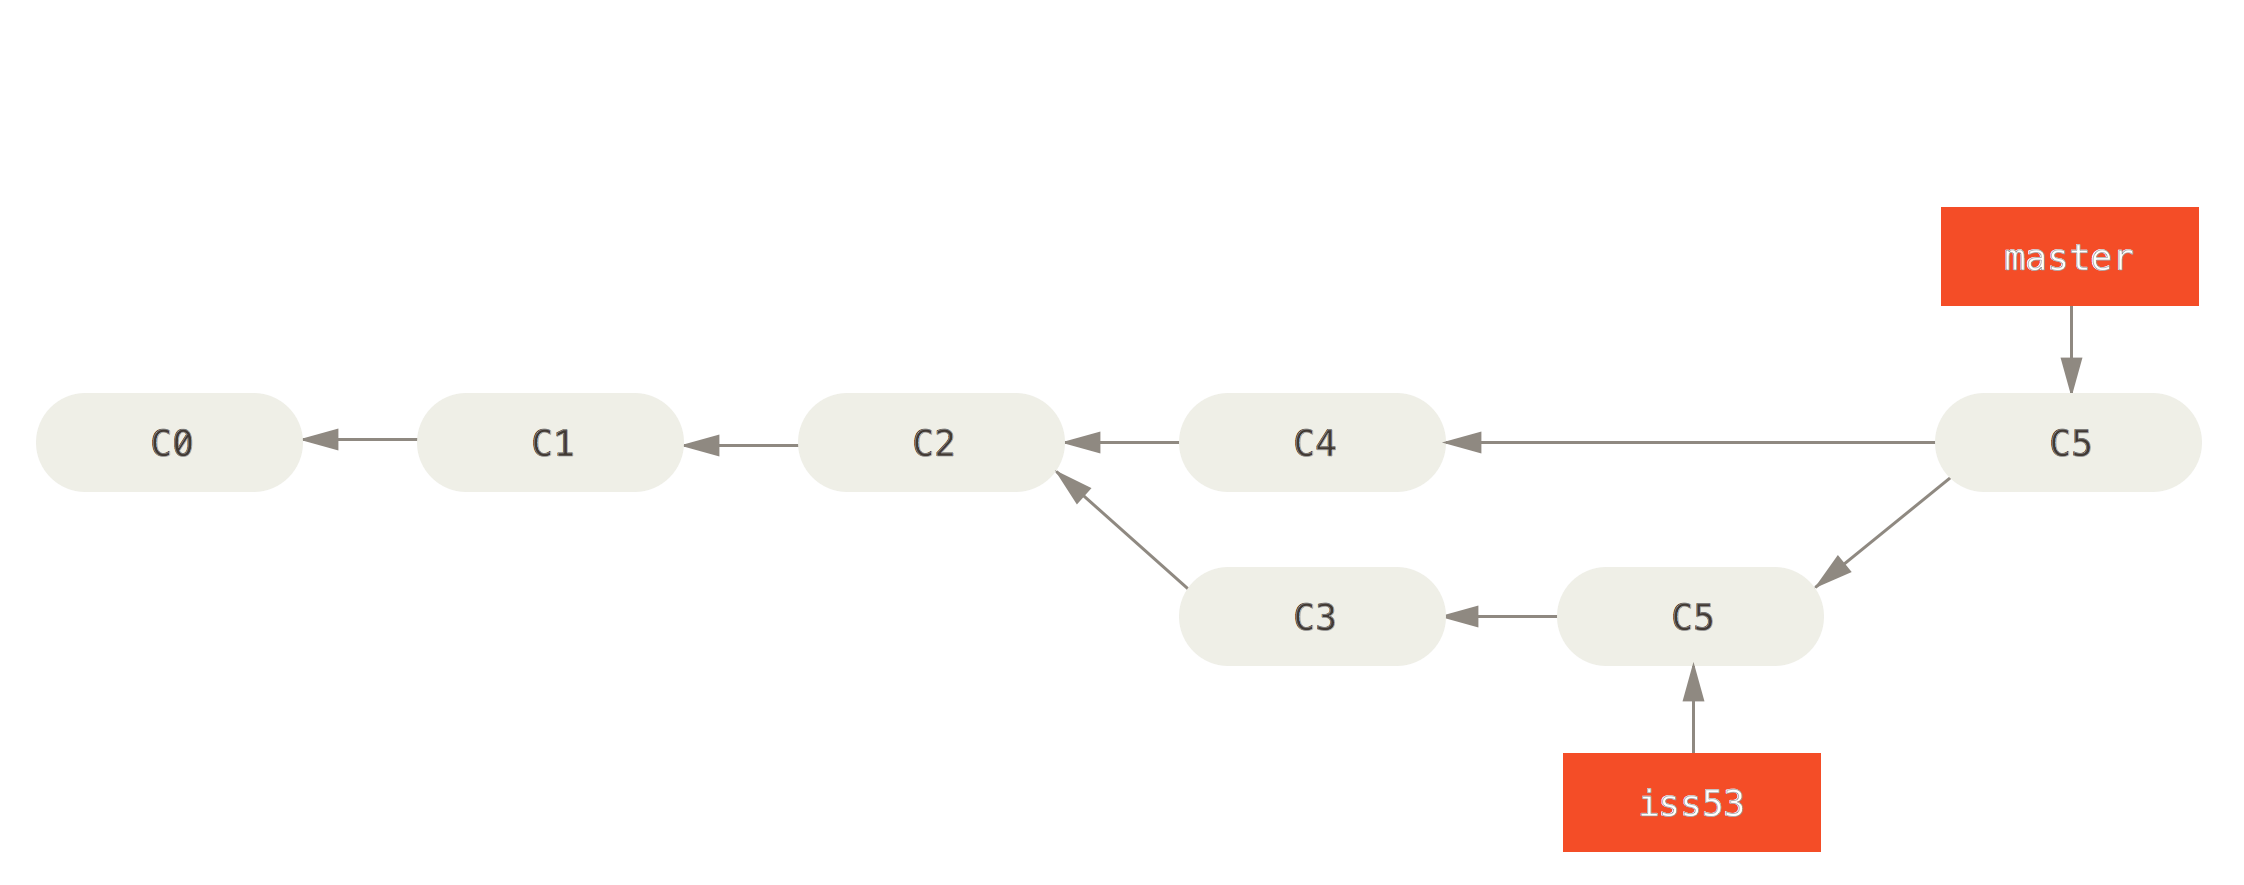
\includegraphics[width=\textwidth]{images/basicbranching}
	\caption{A Simple Branching Scenario \cite{gitbasicbranching}}
	\label{fig:gitbranching}
\end{figure} 

Once work on a branch is complete its changes can be merged into the main branch, or any other branch. When this is done a commit is made, called a 'merge commit' to keep track of the event, in Figure \ref{fig:gitbranching} 'C2' is a merge commit.

\subsection{Forking}
Forking isn't a command in git, or indeed an object type, but rather a concept about how to copy and add to repositories. In the forking workflow \cite{forkingworkflow} a repository is cloned, and committed to as if it was a branch, before pushing changes 'upstream' to the original repository. Often pull requests are required for contributors who do not have direct write access to the original repository.

\section{Existing Git Analysis Tools}
% Section on literature pertaining to accessing git information
	% e.g. http://www.researchgate.net/publication/279058070_Gitana_a_SQL-based_Git_Repository_Inspector
	% Some info on gitinspector
	% Conclusions drawn from the literature
		% Primarily, there isnt many projects doing this. The SQL one has some drawbacks, etc.

\section{Modelling Complex Systems}

\section{Existing Object Model}	
% Section on literature pertaining to analysing and querying git. (there is very little if not none)
	% Conclusions drawn from the literature
		% primarily, its novel
		
		% More in-depth Explanation of Git Object Model
% More in-depth explanation of modelling
	% What is a model?
	% How do we interact with models?
	% etc?

% Section on interacting with object models, or version control software via models. Perhaps the HTML DOM? 

\chapter{Requirements}
% Statement of Needs
% Stakeholder Identification (whos interested in project and their roles)
	% requirements of these stakeholders
% Breakdown of functional (features) and non-functional (speed, UX) requirements
% Use case diagram

\chapter{Methodology}
% Used agile TDD based approach, discuss why this was chosen and

\chapter{Design}
% Making architecture fit between JGit and Epsilon
% Experimentation and changes necessary as things changed (for example learning more about jGit, epsilon and Java or subclassing jGit types to provide better names in EOL code and hide some of the underlying implementation)
% Language
	% Explain how expected EOL code was developed before driver was, so driver could achieve what was wanted  

\chapter{Implementation}
% Environment used
	% Epsilon Eclipse Interim (why interim?)
	% Latest version of Git
% Libraries used
	% JGit
	% Apache Commons Lang
	% etc.
% Projects
	% .git.dt (for creating new Models from git)
	% .git (main functionality of driver)
	% .git.test (tdd stuff)
	% .git.tools (some useful EOL tools for Git stuff)
% Lots of stuff about implementation decisions here
% Summary of what do to to get the system running on your own machine

\chapter{Testing}
% Explain use of TDD, both unit tests, integration and use of EOL files that it would be hoped would work with
% Automated testing
% Use of CI
% Testing against requirements
% Summary (did all test pass?)

\chapter{Evaluation}
% Does it at least fulfil all of the analysis and querying required by the two systems its competing with (github and gitinspector?)
% Case Study vs GitInspector
	% Comparison of lines of code and code complexity required for the same output
	% Comparison of Run Time on same hardware

\chapter{Conclusion}
% Project Review (Cronological rundown of what happened)
% Is this a feasible way of dealing with git analysis and querying?
	% Why? Why not?
% Whats missing?
% A success?


\section{Future Work}
% Currently read only, would be interesting to see if being able to author commits etc via epsilon could be useful. Or even the ability to change names on commits etc via http://stacktoheap.com/blog/2013/01/06/using-mailmap-to-fix-authors-list-in-git/
% Make it would with subversion, mercurial etc
% Transform from git to svn/mercurial or vice versa via ETL (lots of people would want to make this transition)
% Lots of low hanging fruit regarding performance (e.g. computing properties each time instead of storing them in memory once they've been worked out once)

\chapter{Reflection}
% Working on project whilst other 'real life' stuff happens
% Working on coming back to a project after a long time 
% TDD was great, agile working seemed to work well.
% Java code is pretty reasonable, took a little while to get into but previous C# knowledge helped
% Example EOL/EGX code works well, but might be better if more declarative 
% This is one of only a few large projects I've worked on, so it was good experience

\printbibliography

\end{document}
